\documentclass[11pt]{article}

% Packages
\usepackage{graphicx}   % for pictures
\usepackage{amsthm}     % for math
\usepackage{amsmath, mathtools}    %   more math
\usepackage{amsfonts}   %   more math
\usepackage{physics}    % more symbols
\usepackage{circuitikz} % for circuit diagrams
\usepackage{amssymb}    % math symbols
\usepackage{siunitx}    % units
\usepackage{mathrsfs}   % fancy text
\usepackage{color}      % colored letters for notes and reminders
\usepackage{float}      % for image location

%The amsthm package lets you format different types of mathematical ideas nicely. You use it by defining "\newtheorem"s as below:
\newtheorem{problem}{Problem}
\newtheorem{theorem}{Theorem}
\newtheorem*{proposition}{Proposition}
\newtheorem{lemma}[theorem]{Lemma}
\newtheorem{corollary}[theorem]{Corollary}
\theoremstyle{definition}
\newtheorem{defn}[theorem]{Definition}

% Magins

\setlength{\voffset}{0.1in}
\setlength{\paperwidth}{8.5in}
\setlength{\paperheight}{11in}
\setlength{\headheight}{14pt}
\setlength{\headsep}{0.5in}
\setlength{\textheight}{11in}
\setlength{\textheight}{8in}
\setlength{\topmargin}{-0.25in}
\setlength{\textwidth}{7in}
\setlength{\topskip}{0in}
\setlength{\oddsidemargin}{-0.25in}
\setlength{\evensidemargin}{-0.25in}

% For images in this document:
\graphicspath{ {images/} }

% User Defined Commands
\newcommand{\nder}[2]{\frac{d^{#1} #2}{d t^{#1}}}   % The nth derivative wrt t: {n}{x(t)}
\newcommand{\der}[1]{\frac{d #1}{d t}}              % Derivative wrt t: {x(t)}
\newcommand{\infint}{\int_{-\infty}^{\infty}}       % Integral from - infinity to + infinity
\newcommand{\infsum}[1]{\sum_{#1 = -\infty}^{\infty}}% Sum of a variable from - to + infinity
\newcommand{\para}[1]{\left( #1 \right)}            % Instead of writing parenthesis all the time

% User Command for Wider Matrices
\makeatletter
\renewcommand*\env@matrix[1][\arraystretch]{%
  \edef\arraystretch{#1}%
  \hskip -\arraycolsep
  \let\@ifnextchar\new@ifnextchar
  \array{*\c@MaxMatrixCols c}}
\makeatother


% Heading:
\usepackage{fancyhdr}
\pagestyle{fancy}
\lhead{Nicholas Pham}
\chead{ES 155}          %   Change the Class!!
\rhead{Homework 4}   %   Change the Problem Set Number!!


% ----- BEGIN DOCUMENT-----
\begin{document}

\textbf{\huge{ES 155 Homework 4}}    %   Change the Class and Problem Set Number!!
\normalsize

\begin{enumerate}
    \item % Problem 1
    The system model with state variable $x = \begin{bmatrix} c_g \\ c_b \end{bmatrix}$ is

    \begin{align*}
        \dot{x} &= Ax + Bu = \begin{bmatrix} -a_0 - a_1 & a_1 \\ a_2 & - a_2 \end{bmatrix} x + \begin{bmatrix} b_0 \\ 0 \end{bmatrix} u \\
        y &= Cx = \begin{bmatrix} 0 & 1 \end{bmatrix} x
    \end{align*}

    with constants $a_1 = 2$, $a_2 = 1$, $a_0 = 1$, $b_0 = 0.5$.

    \begin{enumerate}
        \item % Part a
        The reachability matrix for a $2 \times 2$ system is given by $w_r = \begin{bmatrix} B & AB \end{bmatrix}$.  Plugging in the given values gives $B = \begin{bmatrix} 0.5 \\ 0 \end{bmatrix}$ and $A = \begin{bmatrix} -3 & 2 \\ 1 & -1 \end{bmatrix}$, so 

        \begin{align*}
            w_r &= \begin{bmatrix} B & AB \end{bmatrix} = \begin{bmatrix} 0.5 & -1.5 \\ 0 & 0.5 \end{bmatrix}
        \end{align*}

        The system is reachable if and only if the reachability matrix is full rank.  In this case, it is easy to see that the row reduced form of the reachability matrix is the identity matrix, so it is full rank.  This shows that the system is reachable.

        \item % Part b
        To determine the controller $u = -Kx + k_r r$, first determine $K = \begin{bmatrix} k_1 & k_2 \end{bmatrix}$.  The goal of the controller is to ensure that the output equals the reference signal $r$, and we know that $\mathtt{eig}(A - BK) = \lambda$ for $\lambda^2 + 2 \zeta_0 \omega_0 \lambda + \omega^2$ for given $\zeta_0$ and $\omega_0$.  The eigenvalues of $(A - BK)$ are computed by $\mathtt{det}(A-BK - I\lambda) = 0$.

        \begin{align*}
            0 &= \mathtt{det}(A-BK - I\lambda) \\
            &= \mathtt{det}\begin{bmatrix} -3 -0.5k_1 - \lambda & 2 - 0.5k_2 \\ 1 & -1 -\lambda \end{bmatrix} \\
            &= \lambda^2 + (4 + 0.5k_1) \lambda + (1 + 0.5k_1 + 0.5k_2) \\
            &= \lambda^2 + 2 \zeta_0 \omega_0 \lambda + \omega^2
        \end{align*}

        This means that

        \begin{align*}
            4 + 0.5k_1 &= 2 \zeta_0 \omega_0 &\implies k_1 &= 4 \zeta_0 \omega_0 - 8\\
            1+ 0.5k_1 + 0.5k_2 &= \omega_0^2 &\implies k_2 &= 2 \omega_0^2 -4 \zeta_0 \omega_0 + 6
        \end{align*}

        Now to find an appropriate $k_r$:

        \begin{align*}
            u &= -Kx + k_r r = -k_1 x_1 - k_2 x_2 + k_r r \\
            \dot{x} &= Ax + Bu = (A - BK)x + B k_r r = \begin{bmatrix} -3 -0.5k_1 & 2 -0.5k_2 \\ 1 & -1 \end{bmatrix} \begin{bmatrix} c_g \\ c_b \end{bmatrix} + \begin{bmatrix} b_0 k_r \\ 0 \end{bmatrix} r
        \end{align*}

        In a steady state, $\dot{x} = 0$, so

        \begin{align*}
            \dot{c_b} &= c_g - c_b  = 0\implies c_b = c_g \\
            \dot{c_g} &= (-3 - 0.5k_1)c_g + (2 - 0.5k_2)c_b + b_0 k_r = 0 \\
            c_b &= \frac{b_0 k_r}{1 + 0.5k_1 + 0.5k_2}r = r \quad \text{from the problem}\\
            k_r &= \frac{1 + 0.5k_1 + 0.5k_2}{b_0} = 2 + k_1 + k_2 = 2 \omega_0^2
        \end{align*}

        Thus, a suitable controller can be written

        \begin{align*}
            u &= -Kx + k_r r = \begin{bmatrix} 4 \zeta_0 \omega_0 - 8 & 2 \omega_0^2 -4 \zeta_0 \omega_0 + 6 \end{bmatrix}x + 2 \omega_0^2 r
        \end{align*}        

        \item % Part c
        See MATLAB code for computing eigenvalues:

        \begin{center}
        \begin{tabular}{c | c c}
            $\zeta_0$ & \multicolumn{2}{c}{$\lambda$} \\
            \hline
            0.1 & $-0.1000 - 0.9950i$ & $-0.1000 + 0.9950i$ \\
            0.4 & $-0.4000 - 0.9165i$ & $-0.4000 + 0.9165i$ \\
            0.7 & $-0.7000 - 0.7141i$ & $-0.7000 + 0.7141i$ \\
            0.9 & $-0.9000 - 0.4359i$ & $-0.9000 + 0.4359i$ \\
        \end{tabular}
        \end{center}

        The step response for the system under the controller from part (b) with these different $\zeta_0$ values is show in Figure \ref{fig:ES155P4_1c_stepResponse}.

        \begin{figure}[!ht]
            \centering
            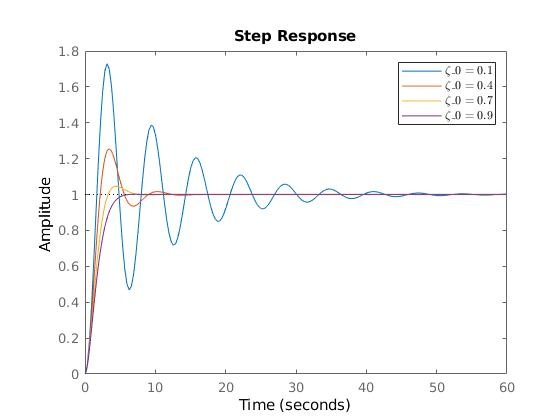
\includegraphics[width = 0.8\textwidth]{ES155P4_1c_stepResponse.jpg}
            \caption{Step response of the system with different parameters $\zeta_0$.}
            \label{fig:ES155P4_1c_stepResponse}
        \end{figure}

        As can be seen, increasing $\zeta_0$ decreases the overshoot, oscillations, and time required for convergence, but decreases the speed at which the output first reaches the target reference.  Even larger values of $\zeta_0$ cause an overdamped response which takes a long time to reach the reference, but do not have any overshoot.  The parameter $\zeta_0$ may be thought of as a damping factor, with critical value perhaps at 1.

        \item % Part d
        As a policy maker, I would want to balance between the adverse health effects of a disease with the costs of medicating the disease.  For instance, an overdamped system in which the patient slowly takes more medicine until they reach their target health might have less economic cost in the short term than taking very powerful drugs quickly that might bring the patient to the desired health in a shorter time.  However, this must be weighed against the physical health costs of the patient being exposed to the disease for a longer time.  There are more nuanced considerations as well: though an underdamped system using less medicine might have a lower short term economic cost, the prolonged exposure to the disease may lead to further complications in the future.  On the other hand, using a strong drug to quickly heal a patient may have other side effects with their own cost.  These effects are dependent on many factors including the nature of the disease, the side effects the drugs might have on the person, as well as different physical parameter values mentioned in the problem.  Clearly, the real world has many variables and complexities than this simple simulation.

        The question of how society should provide the same guarantee for everyone regardless of income level is a somewhat political question.  Individualized care plans taking into account many of the factors described above in addition to income level and personal desires might be a good way to allow for everyone to access at least a plan for care that might be well suited to their interests; emerging AI technologies could be a good fit for implementing such a system.

    \end{enumerate}
    \item % Problem 2

    See MATLAB code for computations.  Use MATLAB's $K = \mathtt{place}(A, B, \{\lambda_0, \ldots \lambda_{n-1}\})$ to find the $K$ matrix. To calculate $k_r$, derive it in the same way from class:

    \begin{align*}
        \dot{x} &= (A - BK)x^* + Bk_rr = 0 \\
        x^* &= -(A-BK)^{-1}Bk_rr \\
        y &= Cx + Du = (C - DK)x + Dk_rr \\
        &= \left( -(C - DK)(a - BK)^{-1}B + D \right)k_rr = r \\
        k_r &= \left( -(C - DK)(a - BK)^{-1}B + D \right)^{-1}
    \end{align*}

    and compute this directly in MATLAB.  Figure \ref{fig:bikeStepResponse} shows the step response to a change in reference angle $r$ from 0 to 0.002 radians.  The figure shows a short period of steering in the opposite direction before settling to the desired angle.  The input torque plot shows a moment of reduced torque during this reverse steering.  The systems tuned with higher magnitude complex eigenvalues show more of this oscillatory behavior, while ones with less magnitude are much more damped.  The bicycle with eigenvalues $\lambda = -2, -10, -5 \pm 5i$ likely feels quite responsive and twitchy to ride.

    \begin{figure}
        \centering
        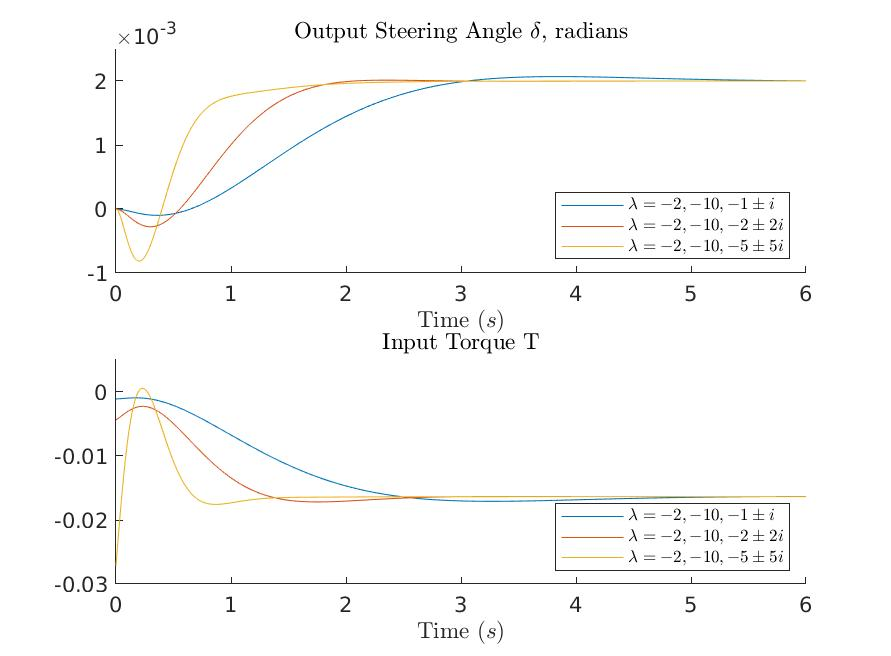
\includegraphics[width = 0.8\textwidth]{ES155P4_2_bicycleStepResponse.jpg}
        \caption{Step response of bicycle to change in desired steering angle for different eigenvalues.}
        \label{fig:bikeStepResponse}
    \end{figure}

\end{enumerate}
\end{document}


